\begin{figure}
\centering
\begin{tikzpicture}
\clip (-6.3,-2.7) rectangle (6.3,2.7);
\node at (-0.07,-0.07) {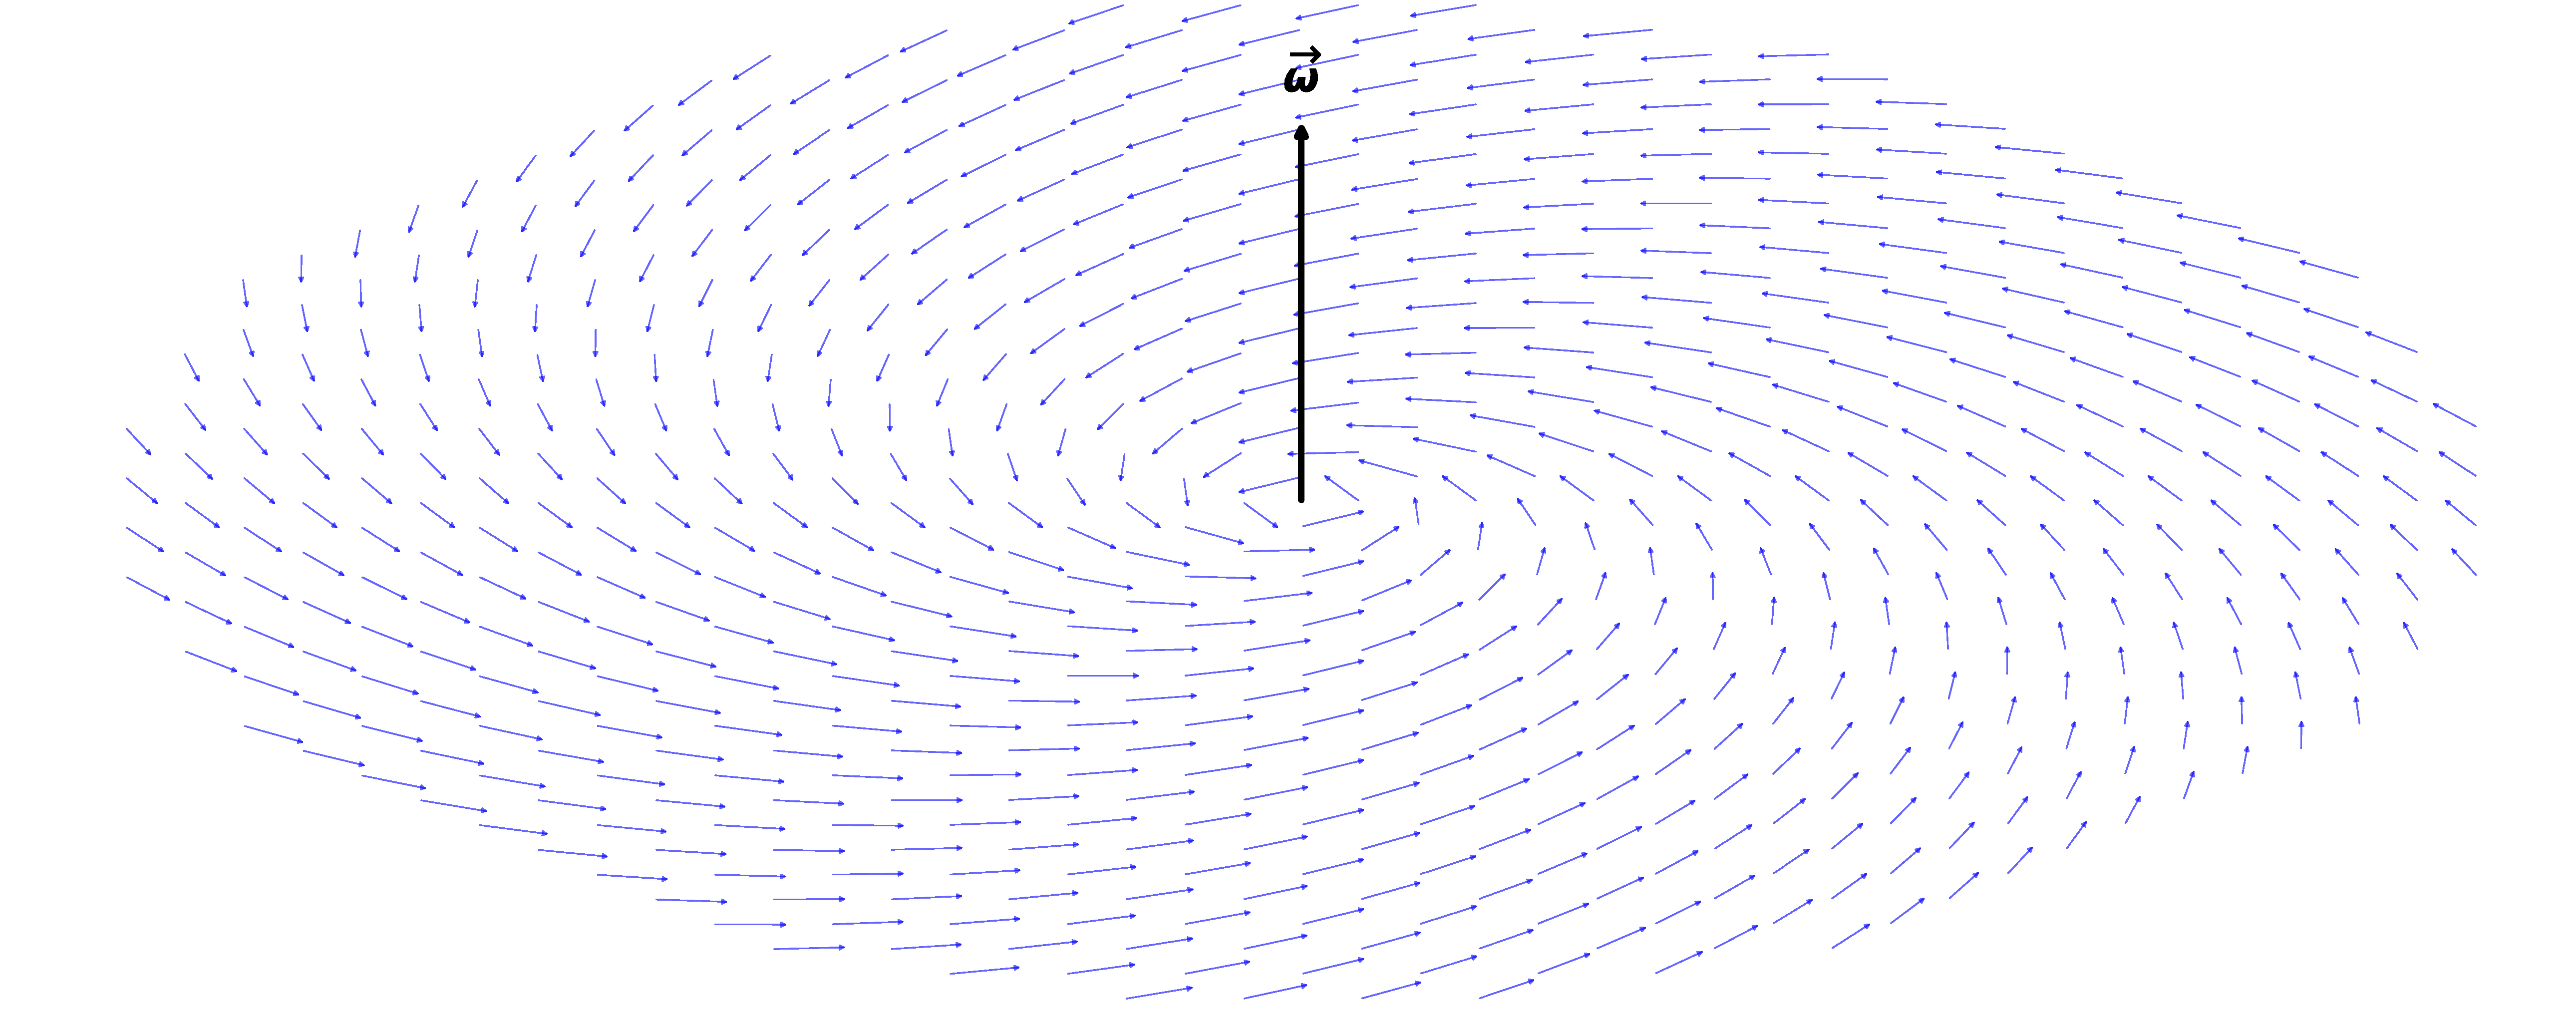
\includegraphics[width=1.08\textwidth]{papers/wirbelringe/fig/flacher_wirbel.pdf}};
%\draw[color=red] (-6.3,-2.7) rectangle (6.3,2.7);
\end{tikzpicture}
\caption{Darstellung eines 2-dimensionalen Wirbels mit Wirbelvektor
\(\vec{\omega}\).
\label{Wirbelringe:fig:flacher_wirbel}}
\end{figure}
